% !Mode:: "TeX:UTF-8"

\chapter{Accelerating FDTD by Using CUDA}

In this chapter, we use the simulation of 2D TM mode as an instance to explain the scheme of accelerating FDTD by using CUDA.

\section{GPU and CUDA}

GPU, is a specialized microprocessor designed to process images rapidly with hundreds of cores and independent memory. The term GPU was popularized by NVIDIA corporation in 1999. GPU was spread with the population of graphic operation systems.

In the early time, for RAM was very expensive, the graphic chips composited data together. Till 80s, the Commondore Amiga featured a custom graphic chip which can manipulate 16-color bitmaps. In 1986, the TMS34010 was released by Texas Instruments, which is the first microprocessor could run general purpose code by using a very graphics-oriented instruction set. OpenGL is a professional graphic application programming interfae (API) appeared in the early 90s, which tried to be a standard cross-language, cross-platform API to rendering 2D and 3D vector graphics. In 2001, the NVIDIA developed the first consumer-level GPU, GeForce 256, which is programmable and supporting OpenGL and DirectX8. In 2006, NVIDIA released CUDA. Against previous API like Direct3D and OpenGL which required advanced skills in graphics programming and advanced understanding of the hardware' architecture, it is designed to work with programming language such as C, C++, and Fortran, which allow people utilize GPU's computation power easier without requiring so much. 

In 2006, NVIDIA released GeForce8800 GTX, which is a milestone of the development of general purpose GPU (GPGPU). From that time, GPU began to have the architecture which suitable to execute general purpose computations, and including several new components like shared memory, multithreading communications which give it the powerful capability of parallel computing.

In 2007, CUDA was unveiled by NVIDIA. Unlike precious generations that partitioned computing resources into vertex and pixel shaders, the CUDA included a unified shader pipeline, which allowing wach and every arithmetic logic unit (ALU) on the chip to be marshaled by a program intending to perform general-purpose computations. Besides, those ALUs were built to comply with IEEE requirements for single-precision floating-point arithmetic and were designed to use an instruction set tailored for general computation rather than specifically for graphics. Furthermore, the execution units on CUDA were allowed arbitrary read and write access to memory as well as access to a sofeware-managed cache known as shared memory. To make the using of GPU more easier, NVIDIA took standard C added a small number of keywords to use GPU. Hence, users are no longer required to have any knowledge of the OpenGL or Direct3D, nor the knowledge to transform their tasks to look like a computer graphics task in order to be executed by GPU.


\section{The Theory of Accelerating FDTD with CUDA}

\subsection{The Programming Model of CUDA}

As GPU is an independent device, so the system of GPU is independent to the system of CPU. Generally, we refer to the CPU and the system's memory as the \textit{host}, and refer to the GPU and its memory as the \textit{device}. The code on host mainly control the work flow of a program, and the code on device often focus on the tasks involving massive computation. 

CUDA allows the programmer to define C functions called \textit{kernels}, which when called, are executed N times in parallel by N different CUDA threads, against only once like regular C functions. When a CUDA program is being executed, kernels are called to use GPU to compute, that is, at first transferring data to GPU, and transferring the result of computing those data back after the tasks are completed. The process is illustrated in Fig. \ref{ch4:cudacallmodel}.

\begin{figure}[hp]
	\centering
	
	%predefine
	\tikzstyle{startstop} = [rectangle, rounded corners, minimum width=3cm, minimum height=1cm,text centered, draw=black]
	\tikzstyle{process} = [rectangle, minimum width=3cm, minimum height=1cm, text centered, draw=black]
	\tikzstyle{arrow} = [thick,->,>=stealth]
	
	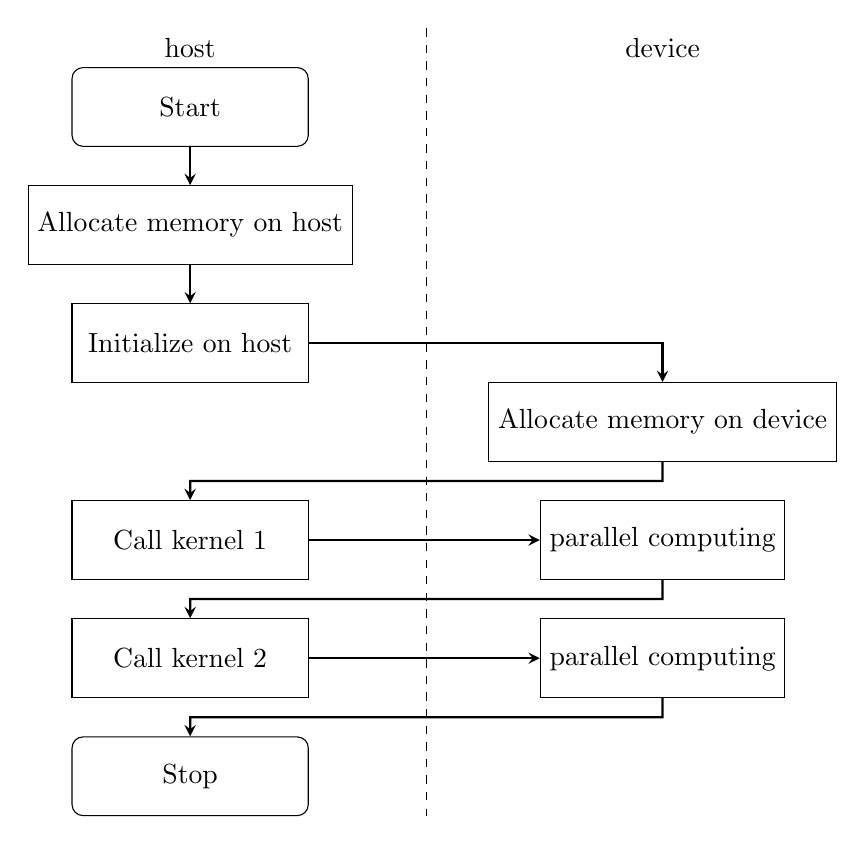
\begin{tikzpicture}
	
	\def \yshift {-0.5cm}
	\def \xshift {5cm}
	
	\draw [dashed] (3,1) -- (3,-9);
	\node (cpu) [above,yshift=-\yshift] {host};
	\node (gpu) [right of=cpu, xshift = \xshift] {device};
	\node (start) [startstop] {Start};
	\node (host alloc) [process, below of=start,yshift=\yshift] {Allocate memory on host};
	\node (host init) [process, below of=host alloc,yshift=\yshift] {Initialize on host};
	\node (device alloc) [process, right of=host init, xshift=\xshift,yshift=2*\yshift] {Allocate memory on device};
	\node (k1) [process, below of=host init, yshift=3*\yshift] {Call kernel 1}; 
	\node (kf1) [process, right of=k1, xshift=\xshift] {parallel computing};
	\node (k2) [process, below of=k1, yshift=\yshift] {Call kernel 2};
	\node (kf2) [process, right of=k2, xshift=\xshift] {parallel computing};
	\node (stop) [startstop, below of=k2,yshift=\yshift] {Stop};
	
	%arrow
	\draw [arrow] (start) -- (host alloc);
	\draw [arrow] (host alloc) -- (host init);
	\draw [arrow] (host init) -| (device alloc);
	\draw [arrow] (device alloc) -- ++(0,1.5*\yshift) -- ++(-6,0) -- (k1);
	\draw [arrow] (k1) --(kf1);
	\draw [arrow] (kf1) -- ++(0,1.5*\yshift) -- ++(-6,0) -- (k2);
	\draw [arrow] (k2) --(kf2);
	\draw [arrow] (kf2) -- ++(0,1.5*\yshift) -- ++(-6,0) -- (stop);
	
	\end{tikzpicture}
	\caption{The process of a CUDA program}
	\label{ch4:cudacallmodel}
\end{figure}

In the following, we will introduce the CUDA programming model by a demonstration to show how to accelerating FDTD with CUDA. In the following code, we write a function which intend to add two vectors.

\begin{lstlisting}
#include "cuda_runtime.h"
#include "device_launch_parameters.h"
#include <stdio.h>
#define N (33 * 1024)
__global__ void add(int *a, const int *b, const int *c)
{
	int tid=threadIdx.x + blockId.x * blockDim.x;
	while(tid < N){
		c[tid] = a[tid] + b[tid];
		tid += blockDim.x * gridDim.x;
	}
}

int main()
{
	//declare for both Host and Device
	int a[N], b[N], c[N];
	int *dev_a, *dev_b, *dev_c;
	
	//allocate memory for Device
	cudaMalloc(&dev_a, N * sizeof(int));
	cudaMalloc(&dev_b, N * sizeof(int));
	cudaMalloc(&dev_c, N * sizeof(int));
	
	//Initialize Host data
	for (int i = 0; i < N; i++){
		a[i] = i;
		b[i] = i * i;
	}
	
	//Transfer Host data to Device.
	cudaMemcpy(dev_a, a, N*sizeof(int), cudaMemcpyHostToDevice);
	cudaMemcpy(dev_b, b, N*sizeof(int), cudaMemcpyHostToDevice);
	
	//Excute Kernel
	add <<<128, 128 >>>(dev_a, dev_b, dev_c);
	
	//Transfer result from Device to Host
	cudaMemcpy(c, dev_c, N*sizeof(int), cudaMemcpyDeviceToHost);
	
	cudaFree(dev_a);
	cudaFree(dev_b);
	cudaFree(dev_c);
	
	return 0;
}
\end{lstlisting}

At first, we define a kernel by using the declaration specifier \lstinline|__global__|, and execution configuration syntax \lstinline|<<<...>>>|, which specify the number of CUDA threads that execute the kernel. Each thread the executes the kernel has a unique thread ID through the built-in \lstinline|threadIdx| variable which can be accessible within the kernel. Before calling a kernel, we should allocate memory on device first for three arrays. Correspondingly, we should free the memory allocated when they are no longer needed. Besides, as we mentioned before, the memories of device and host are independent, so we need transfer the data waited to be manipulated to kernel before calling it and transfer the computing result after the kernel being called.

\subsection{Thread Hierarchy}

The basic unit of parallel computing is thread. As mentioned above, thread had its own \lstinline|threadIdx|, a 3-component vector. So, we can identify thread by using a one-dimensional, two-dimensional, or three-dimensional thread index, to from a one-dimensional, two-dimensional, ot three-dimensional block of threads, called a thread block. The threads in the same thread block can share memory and communicate with each other rapidly. The number of block and threads per block has is defined by arguments in \lstinline|<<<...>>>|. The first argument in the chevrons specify the number of thread blocks, and the second argument specify the number of threads per thread block has. In the sample code above, the host code in line 36 invoke 128 thread blocks with 128 threads per thread block. The GPU will create a copy of function \lstinline|add()| for each thread and process them in a parallel way.

In the line 7 of the sample code, there are some built-in variables, which is \lstinline|threadIdx.x|, \lstinline|blockId.x|, and \lstinline| blockDim.x|. For those built-in variables, there is no need to define it or assign a value to it. It contains the value of the index or the size for a thread or block. For a two-dimensional block of size $(D_x, D_y)$, the thread ID of a thread of index $(x,y)$ is $(x+yD_x)$; for a three-dimensional block of size $(D_x,D_y,D_z)$, the thread ID of a thread of index $(x,y,z)$ is $(x+yD_x+zD_x D_y)$. In the Fig. \ref{ch4:grid and thread}, we illustrate the relationship between a two-dimensional block with threads it has.

\begin{figure}[hp]
	\centering
	\begin{tikzpicture}
	\def \len {2}
	\def \hl {1}
	
	\node at (-\hl,\len) {Thread block};
	%1
	\draw[fill=cyan](0,0) rectangle +(\len,\len); \node at ($0.5*(\len,\len)$) {$(0,0)$};
	\draw($(\len,0)$) rectangle +(\len,\len);\node at ($(\len,0)+0.5*(\len,\len)$) { $(0,1)$};
	\draw($(2*\len,0)$) rectangle +(\len,\len);\node at ($(2*\len,0)+0.5*(\len,\len)$) { $(0,2)$};
	
	%2
	\draw(0,\len) rectangle +(\len,\len);\node at ($(0,\len)+0.5*(\len,\len)$) { $(1,0)$};
	\draw($(\len,\len)$) rectangle +(\len,\len);\node at ($(\len,\len)+0.5*(\len,\len)$) { $(1,1)$};
	\draw($(2*\len,\len)$) rectangle +(\len,\len);\node at ($(2*\len,\len)+0.5*(\len,\len)$) { $(1,2)$};
	
	%thread
	\draw ($(\hl,3*\len)$) rectangle +($(\hl,\hl)$);
	\node at ($(0.5*\len,3*\len)+0.5*(\hl,\hl)$) {$(0,0)$};
	\draw ($(2*\hl,3*\len)$) rectangle +($(\hl,\hl)$);
	\node at ($(2*\hl,3*\len)+0.5*(\hl,\hl)$) {$(0,1)$};
	\draw ($(3*\hl,3*\len)$) rectangle +($(\hl,\hl)$);
	\node at ($(3*\hl,3*\len)+0.5*(\hl,\hl)$) {$(0,2)$};
	\draw ($(4*\hl,3*\len)$) rectangle +($(\hl,\hl)$);
	\node at ($(4*\hl,3*\len)+0.5*(\hl,\hl)$) {$(0,3)$};
	
	\draw ($(\hl,3*\len+\hl)$) rectangle +($(\hl,\hl)$);
	\node at ($(0.5*\len,3*\len+\hl)+0.5*(\hl,\hl)$) {$(1,0)$};
	\draw ($(2*\hl,3*\len+\hl)$) rectangle +($(\hl,\hl)$);
	\node at ($(2*\hl,3*\len+\hl)+0.5*(\hl,\hl)$) {$(1,1)$};
	\draw ($(3*\hl,3*\len+\hl)$) rectangle +($(\hl,\hl)$);
	\node at ($(3*\hl,3*\len+\hl)+0.5*(\hl,\hl)$) {$(1,2)$};
	\draw ($(4*\hl,3*\len+\hl)$) rectangle +($(\hl,\hl)$);
	\node at ($(4*\hl,3*\len+\hl)+0.5*(\hl,\hl)$) {$(1,3)$};
	
	%dashed
	\draw [dashed] (0,0) -- +($(0.5*\len,3*\len)$);
	\draw [dashed] (0,\len) -- +($(0.5*\len,3*\len)$);
	\draw [dashed] (\len,0) -- +($(1.5*\len,3*\len)$);
	\draw [dashed] (\len,\len) -- +($(1.5*\len,3*\len)$);
	
	\end{tikzpicture}
	\caption{The relation between a two-dimensional thread block and threads it has}
	\label{ch4:grid and thread}
\end{figure}

After all threads finished their copy of kernel, we add the theirs index with the number of all threads in all blocks, like what line 10 doing in the sample code. By doing this, we can compute vectors in arbitrary size with finite number of threads and blocks.

\section{The Scheme of Accelerating FDTD with CUDA}

Before we consider the scheme of kernels, we think some optimizations for auxiliary work.

First, we consider the transfer step. As mentioned above, before calling a kernel, we need transfer the data which need to be manipulated to device, and transfer the result back to host. This process will bring us some inconveniences.

The transfer step is accomplished in a serial way, which is inefficient, especially considering that almost all kernel need to handle massive data and the limitation of the I/O capability of hardwares, thus the CPU and GPU will have a long time with nothing meaningful to do, wasting their power of computation. 

For this problem, we adopt a measure that instead of transfer data from host to device, we initialize data on device directly after allocating memory on it. By doing this, half time of transferring data is saved.

Second, we consider the memory of device. Considering we need to have a 2D arrays' allocations, we performing pitch allocations using \lstinline|cudaMallocPitch| instead of \lstinline|cudaMalloc|. The alignment in memory had been mentioned in the chapter 2 that if the allocations are not aligned much time would be wasted on accessing memory and loading data. The \lstinline|cudaMallocPitch| ensure that the starting address of each row in a 2D array is a multiple of $2^N$, where $N$ is 7\~10. In the worst condition, the time can be 1.5 times of not aligned condition compared to the aligned condition. For the same reason, we use \lstinline|cudaMemcpy2D| instead of \lstinline|cudaMemcpy| to get the result back from device to host.

Together with the optimizations mentioned above, we draw the framework of FDTD program, which shown in Fig. \ref{ch4:prog consitit}. There are two parts of the CUDA program, one part is classes, and another is functions. In the classed part, three classed are defined. The members of class \lstinline|E| include the information of electric field, and some method like initialization, checking, and saving the data of electric field in files. The class \lstinline|H|, like class, define the same thing to the $H_x$ and $H_y$ field components. The class \lstinline|src|, on the other hand, specify the information and methods of the whole simulation area, including the excitation source, the scale of Yee cells, the number of time steps, etc.

The function part, also the key part of the program, is responsible to the process of updating values of each discrete field point, including the updating of magnetic field points, the updating of electric field point, and the process of boundary condition in each tiem step.

\begin{figure}[hp]
	\centering
	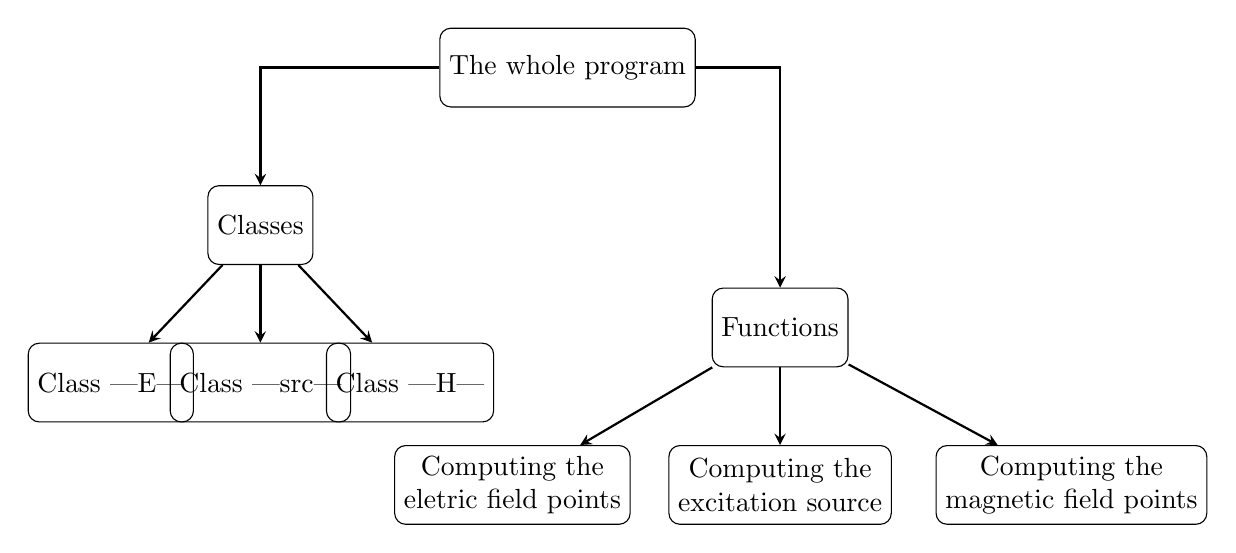
\begin{tikzpicture}
		\tikzstyle{box} = [rectangle, rounded corners, minimum width = 1cm, minimum height=1cm,text centered, draw=black,align=center]
		\tikzstyle{arrow} = [thick,->,>=stealth]
		\def \xshift {3cm}
		\def \yshift {-1cm}
		
		\node (whole) [box] {The whole program};
		\node (class) [box, below of=whole,xshift = -1.3*\xshift, yshift=\yshift] {Classes};
		\node (func) [box, below of =whole, xshift = 0.9*\xshift, yshift=2.3*\yshift] {Functions};
		%class
		\node (src) [box, below of=class, yshift=\yshift] {Class \lstinline|src|};
		\node (E) [box, left of=src, xshift=-0.3*\xshift] {Class \lstinline|E|};
		\node (H) [box, right of=src, xshift=0.3*\xshift] {Class \lstinline|H|};
		%function
		\node (cmpsrc) [box, below of=func,yshift = \yshift] {Computing the \\excitation source};
		\node (cmph) [box, right of=cmpsrc, xshift=0.9*\xshift] {Computing the \\magnetic field points};
		\node (cmpe) [box, left of=cmpsrc, xshift=-0.8*\xshift] {Computing the \\eletric field points};
		
		\draw [arrow] (whole) -| (class);
		\draw [arrow] (whole) -| (func);
		\draw [arrow] (class) -- (src);
		\draw [arrow] (class) -- (E);
		\draw [arrow] (class) -- (H);
		\draw [arrow] (func) -- (cmpsrc);
		\draw [arrow] (func) -- (cmph);
		\draw [arrow] (func) -- (cmpe);
	\end{tikzpicture}
	\caption{The framework of FDTD program with using CUDA}
	\label{ch4:prog consitit}
\end{figure}

The work flow of the program if shown in Fig. \ref{ch4: workflow}. At the beginning we initialize the simulation area, plus the class \lstinline|E| and \lstinline|E|. Then we step into the loop of updating values of each discrete field point. After the loop the program get the result back from device and write the information of field components in files. At last, free the allocations of memory and end the program. The code is in following:
\begin{lstlisting}
src source(4000, 1000, 1000);
H Hxy(source);
E Ez(source);
int i;

for (i = 0; i < source.size_time; i++){
	Hy_cmp_kernel << <50, 50 >> >(Ez.dev_Ez, Hxy.dev_Hy, Hxy.size_Hy_x, Hxy.size_Hy_y, Hxy.coe_H, Ez.ele_Ez, Hxy.ele_Hy);
	Hx_cmp_kernel << <50, 50 >> >(Ez.dev_Ez, Hxy.dev_Hx, Hxy.size_Hx_x, Hxy.size_Hx_y, Hxy.coe_H, Ez.ele_Ez, Hxy.ele_Hy);
	Ez_cmp_kernel << <50, 50 >> >(Ez.dev_Ez, Hxy.dev_Hx, Hxy.dev_Hy, Ez.coe_Ez, Ez.size_Ez_x, Ez.size_Ez_y, Ez.ele_Ez, Hxy.ele_Hx, Hxy.ele_Hy);
	Ez_MUR_u << <50, 50 >> >(Ez.dev_Ez, Ez.E_bd_u, Ez.E_nbd_u, Ez.size_Ez_x, Ez.size_Ez_y, Ez.coe_MUR, Ez.ele_Ez);
	Ez_MUR_d << <50, 50 >> >(Ez.dev_Ez, Ez.E_bd_d, Ez.E_nbd_d, Ez.size_Ez_x, Ez.size_Ez_y, Ez.coe_MUR, Ez.ele_Ez);
	Ez_MUR_lr << <1, Ez.size_Ez_y >> >(Ez.dev_Ez, Ez.E_bd_l, Ez.E_nbd_l, Ez.E_bd_r, Ez.E_nbd_r, Ez.size_Ez_x, Ez.size_Ez_y, Ez.coe_MUR, Ez.ele_Ez);
	src_cmp_kernel << <1, 1 >> >(i, Ez.dev_Ez, Ez.size_Ez_x, Ez.size_Ez_y, source.dt, Ez.ele_Ez);

	cudaMemcpy2D(Ez.Ez, Ez.size_Ez_x*sizeof(float), Ez.dev_Ez, Ez.pitch_Ez, Ez.size_Ez_x*sizeof(float), Ez.size_Ez_y, cudaMemcpyDeviceToHost);
}
\end{lstlisting}

\begin{figure}[hp]
	\centering
	\tikzstyle{startstop} = [rectangle, rounded corners, minimum width=3cm, minimum height=1cm,text centered, draw=black]
	\tikzstyle{process} = [rectangle, minimum width=3cm, minimum height=1cm, text centered, draw=black,align=center]
	\tikzstyle{arrow} = [thick,->,>=stealth]
	\tikzstyle{decision} = [diamond, shape aspect=2,minimum width=3cm, minimum height=1cm, text centered, draw=black]
	\tikzstyle{io} = [trapezium, trapezium left angle=70, trapezium right angle=110, minimum width=3cm, minimum height=1cm, text centered, draw=black,align=center]
	\begin{tikzpicture}
		
		
		\def \yshift {-1cm}
		\def \xshift {5cm}
		
		\node (start) [startstop] {Start};
		\node (init) [io, below of=start, yshift=\yshift] {Initializing the field points\\and simulation area};
		\node (fdtdarea) [process,below of=init,yshift=\yshift] {Updating the values of field points};
		\node (bd) [process,below of=fdtdarea,yshift=\yshift] {Processing Mur ABC};
		\node (trans) [process, below of = bd, yshift=\yshift] {Getting the result back from device to host};
		\node (save) [io, below of =trans, yshift=\yshift] {Saving the values\\of field components};
		\node (judge) [decision,below of=save,yshift=2*\yshift] {Judging if the loop finished};
		\node (stop) [startstop,below of=judge,yshift=1.5*\yshift] {Stop};
		
		\draw [arrow] (start)--(init);
		\draw [arrow] (init)--(fdtdarea);
		\draw [arrow] (fdtdarea)--(bd);
		\draw [arrow] (bd)--(trans);
		\draw [arrow] (trans)--(save);
		\draw [arrow] (save)--(judge);
		\draw [arrow] (judge)--node[anchor=east] {Yes} (stop);
		\draw [arrow] (judge) --node[anchor=south] {No} ++(\xshift,0) |- (fdtdarea);
		
	\end{tikzpicture}
	\caption{The work flow of program}
	\label{ch4: workflow}
\end{figure}

In the process of updating values, we adopt a way following the programming model discussed above. Taking the code of updating process of $E_z$ shown in the following as an example:
\begin{lstlisting}
__global__
void Ez_cmp_kernel(
float* Ez, float* Hx, float* Hy,
float coe_Ez, int size_Ez_x, int size_Ez_y,
int ele_ex, int ele_hx, int ele_hy
)
{
	int x, y;
	int tid, number;
	tid = threadIdx.x + blockIdx.x*blockDim.x;
	float dif_Hy, dif_Hx;
	while (tid < ele_ex*size_Ez_y)
	{
		number = tid + 1;
		y = number % ele_ex;//row
		x = number - (y*ele_ex);//column
		//Hy(i,j)	-	Hy(i-1,j)
		dif_Hy = Hy[y*ele_hy + x] - Hy[(y - 1)* ele_hy + x];
		//Hx(i,j-1)	-	Hx(i,j)
		dif_Hx = Hx[y*ele_hx + (x - 1)] - Hx[y*ele_hx + x];
		Ez[y*ele_ex + x] += coe_Ez * (dif_Hx + dif_Hy);
		tid += blockDim.x*gridDim.x;
	}
}
\end{lstlisting}

For each copy of a thread, we calculate the coordinate of the discrete field point the thread process. Then we find corresponding discrete field point according to the coordinate we have and the updating formulations explicated in chapter 2. In the line 22, we assign the thread which has done a copy of kernel to manipulate another copy of kernel, until all discrete field points have been processed.

\section{Simulation Result}
In the Fig. \ref{ch4 fig:sCUDA} we illustrate the simulation result of FDTD. 

\begin{figure}
	\centering
	\begin{minipage}{0.47\textwidth}
		\centering
		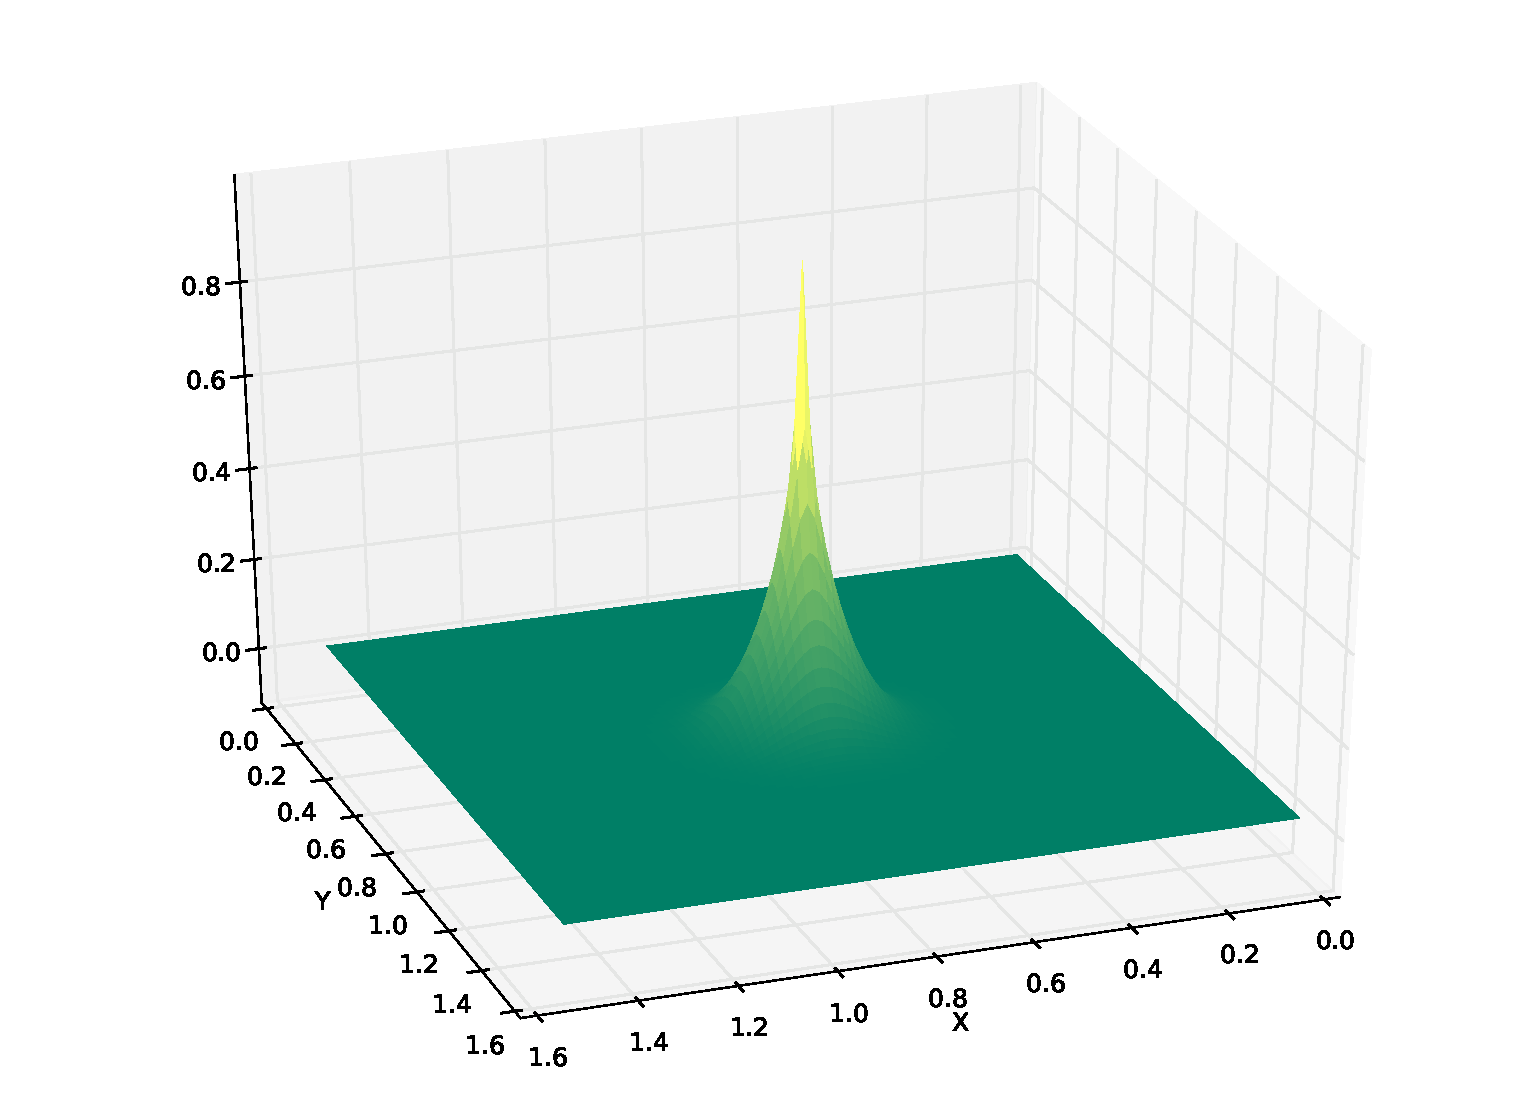
\includegraphics[width=\textwidth]{s1}
	\end{minipage}
	\begin{minipage}{0.47\textwidth}
		\centering
		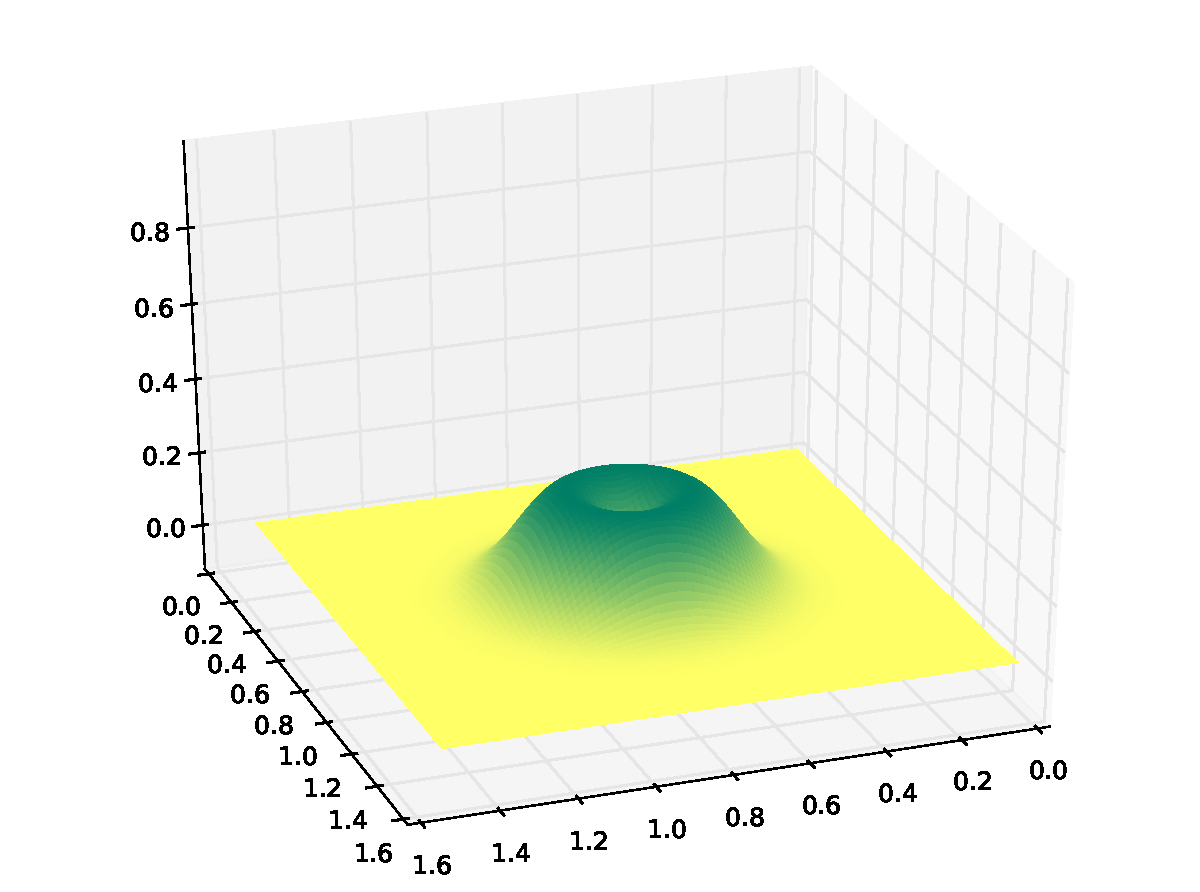
\includegraphics[width=\textwidth]{s2}
	\end{minipage}
	\newline
	\begin{minipage}{0.47\textwidth}
		\centering
		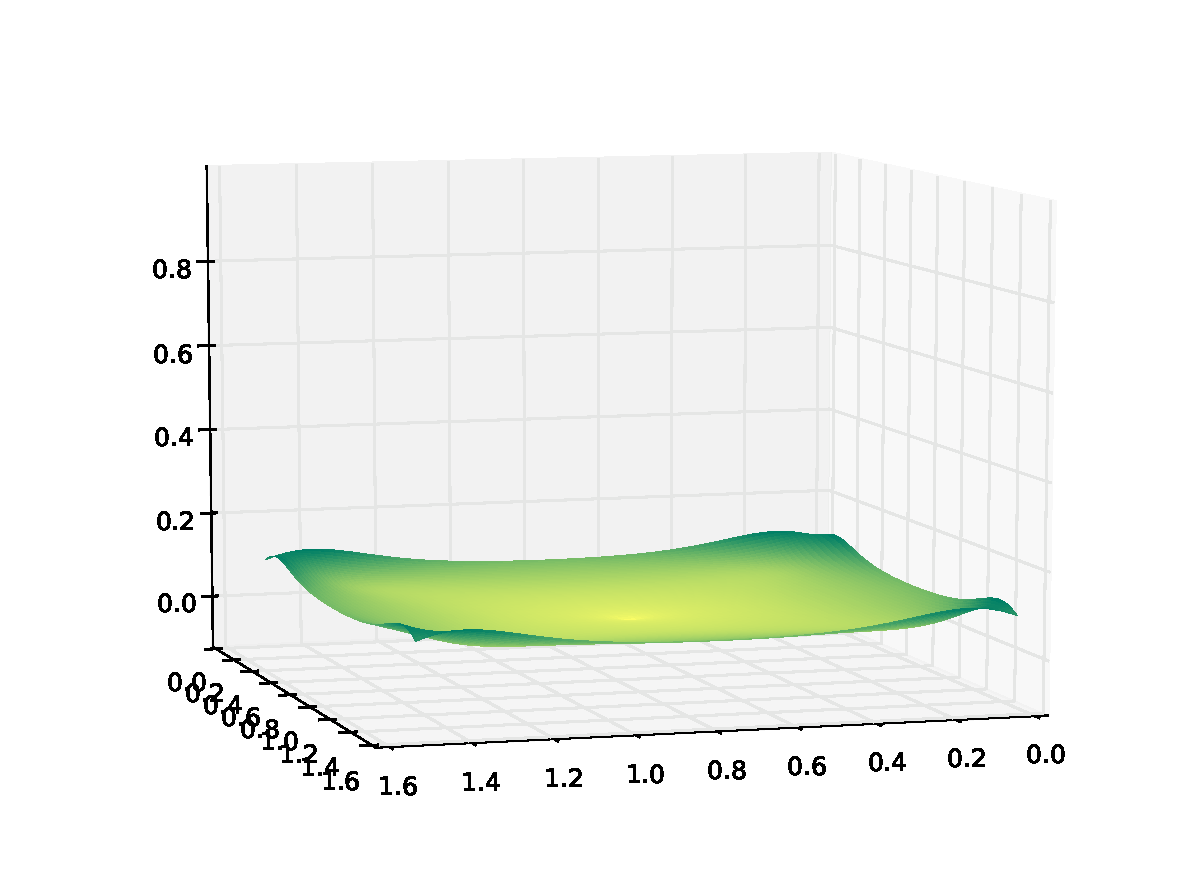
\includegraphics[width=\textwidth]{s3}
	\end{minipage}
	\begin{minipage}{0.47\textwidth}
		\centering
		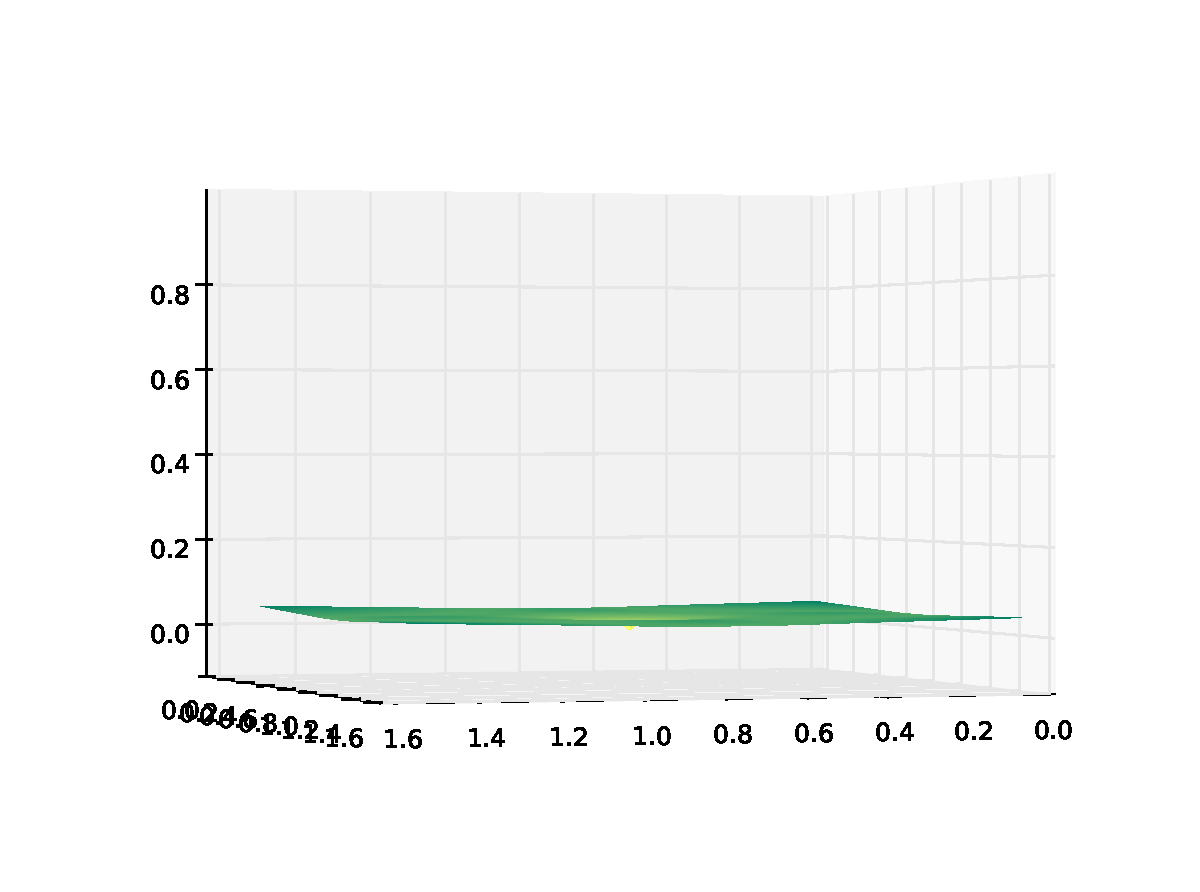
\includegraphics[width=\textwidth]{s4}
	\end{minipage}
	\centering
	\caption{The simulation result of the FDTD with CUDA scheme}
	\label{ch4 fig:sCUDA}
\end{figure}

From Fig. \ref{ch4 fig:sCUDA}, we can see the simulation was successful: the electromagnetic wave was absorbed on the boundaries.

\section{The performance of FDTD with CUDA}

Here, we also take the computation of 2D FDTD TM wave using Mur ABC as an example to analyze the difference of performance between FDTD without data parallelism, the modified method with VP, and FDTD with CUDA in different space and time sizes. Furthermore, we analyze the efficiency of those two methods based on those results.

The call tree view of program is as what Fig. \ref{ch4:call tree} showing. We also adopt the profiling methods used in chapter 3. The following tables present the profiling reports.

\begin{figure}[hp]
	\centering
	\begin{tikzpicture}
		\tikzstyle{box} = [rectangle, rounded corners, minimum width = 1cm, minimum height=1cm,text centered, draw=black,align=center]
		\tikzstyle{arrow} = [thick,->,>=stealth]
		\def \xshift {4cm}
		\def \yshift {-1cm}
		
		\node (main) [box] {\lstinline|main|};
		\node (keycmp) [box,right of=main,yshift=-\yshift,xshift=\xshift] {Key computing functions};
		\node (mincmp) [box,right of=main,yshift=2.1*\yshift,xshift=\xshift] {Other computing functions};
		\node (init) [box,above of=keycmp,yshift=-2.7*\yshift] {Initialization functions};
		\node (otherfunc) [box,below of=mincmp,yshift=1.1\yshift] {Other functions};
		
		\draw [arrow] (main) --++(0.5*\xshift,0)-- +(0,-4.7*\yshift)--(init);
		\draw [arrow] (main) --++(0.5*\xshift,0)-- +(0,-1*\yshift)--(keycmp);
		\draw [arrow] (main) --++(0.5*\xshift,0)-- +(0,2.1*\yshift)--(mincmp);
		\draw [arrow] (main) --++(0.5*\xshift,0)-- +(0,4.1*\yshift)--(otherfunc);
		
		\node (src) [box,right of=init,xshift=\xshift] {\lstinline|src::src|};
		\node (Hxy) [box,above of=src,yshift=-0.2*\yshift] {\lstinline|Hxy::Hxy|};
		\node (E) [box,below of=src,yshift=0.2*\yshift] {\lstinline|E::E|};
		\draw [arrow] (init) -- (src);
		\draw [arrow] (init) -- (Hxy);
		\draw [arrow] (init) -- (E);
		
		\node (hxcmp) [box,right of=keycmp,xshift=\xshift] {\lstinline|Hx_cmp_kernel|};
		\node (hycmp) [box,above of=hxcmp,yshift=-0.2*\yshift]
		 {\lstinline|Hy_cmp_kernel|};
		\node (ezcmp) [box,below of=hxcmp,yshift=0.2*\yshift] {\lstinline|Ez_cmp_kernel|};
		\draw [arrow] (keycmp) -- (hxcmp);
		\draw [arrow] (keycmp) -- (hycmp);
		\draw [arrow] (keycmp) -- (ezcmp);
		
		\node (bd) [box,right of=mincmp,yshift=-0.6*\yshift,xshift=\xshift] {The Mur ABC\\processing function};
		\node (srccmp) [box,right of=mincmp,xshift=\xshift,yshift=0.7*\yshift] {\lstinline|src_cmp_kernel|};
		\draw [arrow] (mincmp)--(bd);
		\draw [arrow] (mincmp)--(srccmp);
		
		\node (other) [box,right of=otherfunc,xshift=\xshift] {Auxiliary functions};
		\draw [arrow] (otherfunc) -- (other);
		
		
	\end{tikzpicture}
	\caption{The call tree view of program}
	\label{ch4:call tree}
\end{figure}

\begin{table}[hp]
	\centering
	\begin{threeparttable}
		\caption{The comparison between serial way and using CUDA}\label{ch4: cuda or not}
		\begin{tabular}{cccc}
			\toprule
			\multirow{2}{2em}{Function}&\multicolumn{2}{c}{Elapsed Inclusive (ms)} & \multirow{2}{14em}{The time saved by using CUDA}\\
			\cline{2-3}
			& serial way & using CUDA & \\ 
			
			\midrule
			\lstinline|main| & 10330.43 & 888.30 & 91.4\% \\
			\lstinline|H_cmp|\tnote{3} & 6.16 &  & \\ 
			\lstinline|E_cmp|\tnote{3} & 4.10 &  & \\
			\lstinline|Hy_cmp_kernel|\tnote{4} &  & $<$0.01 & \\ 
			\lstinline|Hx_cmp_kernel|\tnote{4} &  & $<$0.01 & \\ 
			\lstinline|Ez_cmp_kernel|\tnote{4} &  & $<$0.01 & \\
			\bottomrule
		\end{tabular} 
		\begin{tablenotes}
			\item[1] The size of simulation area is 2000$\times$1000 Yee cells.
			\item[2] The number of time step is 1000.
			\item[3] Only in serial way.
			\item[4] Onely in the way of using CUDA.
		\end{tablenotes}
	\end{threeparttable}
\end{table}

The Table \ref{ch4: cuda or not} represent the performances of using serial way and using CUDA. What we can see from it is the time elapsed by computational functions, ie $H\_cmp$ and $E\_cmp$ takes significant part of the whole time in the serial way, but takes only less than 1\% of the whole time in using CUDA way. In fact, in the CUDA accelerating scheme, in each time step, for each discrete field points we use a individual thread to execute it, which means that all values of points are updated at the same time. In theory, if the number of threads in all thread blocks is $Sum_{thrd}$, the time used in computation by using CUDA is $1/Sum_{thrd}$ times of it in serial way. From the profiling report we also can see that, the time used to update values of filed points takes only 0.81\%, and almost all time were taken to allocate memory.

\begin{table}[hp]
	\centering
	\caption{The comparison between the modified data parallelism and using CUDA}\label{ch4: cuda or new}
\begin{threeparttable}
	\begin{tabular}{cccc}
		\toprule
		\multirow{2}{2em}{Function}&\multicolumn{2}{c}{Elapsed Inclusive (ms)} & \multirow{2}{14em}{The time saved by using CUDA}\\ 
		\cline{2-3}
		& \makecell{The modified\\data parallelism} & Using CUDA & \\ 
		
		\midrule
			\lstinline|main| & 7835.78 & 888.30 & 88.67\% \\
			\lstinline|H_cmp|\tnote{3} & 4.64 &  & \\ 
			\lstinline|E_cmp|\tnote{3} & 3.13 &  & \\
			\lstinline|Hy_cmp_kernel|\tnote{4} &  & $<$0.01 & \\ 
			\lstinline|Hx_cmp_kernel|\tnote{4} &  & $<$0.01 & \\ 
			\lstinline|Ez_cmp_kernel|\tnote{4} &  & $<$0.01 & \\
		\bottomrule
	\end{tabular}
	\begin{tablenotes}
		\item[1] The size of simulation area is 2000$\times$1000 Yee cells.
		\item[2] The number of time step is 1000.
		\item[3] Only in serial way.
		\item[4] Onely in the way of using CUDA.
	\end{tablenotes}
\end{threeparttable}
\end{table}

The Table \ref{ch4: cuda or new} represent the comparison between data parallelism and CUDA. From the comparison we can know that the time taken by updating values is still less than 1\%.

\begin{table}[hp]
	\centering
	\begin{threeparttable}
		\caption{The performance of CUDA under different size of simulation area}\label{ch4: cuda, size}
		\begin{tabular}{cccc}
			\toprule
			\multirow{2}{2em}{Function}&\multicolumn{3}{c}{Elapsed Inclusive (ms)}\\ 
			\cline{2-4}
			$2000\times1000$ & $3000\times1000$ & $4000\times1000$\\ 
			
			\midrule
			\lstinline|main| & 883.30 & 923.67 & 942.05\\
			\lstinline|Hy_cmp_kernel| & $<$0.01 & $<$0.01 & $<$0.01\\ 
			\lstinline|Hx_cmp_kernel| & $<$0.01 & $<$0.01 & $<$0.01\\ 
			\lstinline|Ez_cmp_kernel| & $<$0.01 & $<$0.01 & $<$0.01\\
			\bottomrule
		\end{tabular}
		\begin{tablenotes}
			\item[1] The number of time step is 1000.
		\end{tablenotes}
	\end{threeparttable}
\end{table}

In Table \ref{ch4: cuda, size} we can see that even the size of simulation area increase, the time used to update values is still very short, even too short to measure it. Compared to the Table \ref{ch4: cuda or new}, it is obviously that even accelerate by VP, the execution is still slow in hundreds times compared to using CUDA.

\begin{table}[hp]
	\centering
	\begin{threeparttable}
		\caption{The performance of CUDA under different number of time steps}\label{ch4: cuda, time}
		\begin{tabular}{c>{\centering}p{10em}p{8em}}
			\toprule
			\multirow{2}{6em}{Function}&\multicolumn{2}{c}{Elapsed Inclusive (ms)}\\ 
			\cline{2-3}
			& 1000 time steps & 3000 time steps\\ 
			
			\midrule
			\lstinline|main| & 833.30 & 1139.94 \\ 
			\lstinline|Hy_cmp_kernel| & $<$0.01 & $<$0.01 \\ 
			\lstinline|Hx_cmp_kernel| & $<$0.01 & $<$0.01\\ 
			\lstinline|Ez_cmp_kernel| & $<$0.01 & $<$0.01\\
			\bottomrule
		\end{tabular}
		\begin{tablenotes}
			\item[1] The size of simulation area is 2000$\times$1000 Yee cells.
		\end{tablenotes}
	\end{threeparttable}
\end{table}

From Table \ref{ch4: cuda, time}, we can see that in different number of time iterations, the CUDA scheme can also accomplish the computational task in a very short time. From the profiling report, we can know that the differences in elapsed time between those different conditions are caused by the function \lstinline|cudaMallocPitch|, which need to allocate memory for arrays. This function, takes about 90\% time of the whole time. No more details revealed by NVIDIA corporation so far, so we do not understand the reason behind this situation.

\section{Conclusion}

In this chapter, we introduced the architecture of CUDA, and the programming model used to accelerating FDTD with using CUDA. Then we explicate our CUDA scheme, which taking the computation of 2D FDTD TM wave using Mur ABC as an example, and profiling the performance of our scheme. Furthermore, we analyze the profiling reports together the reports given in previous chapters. In the analysis, we found that the potential of CUDA is substantial. However, we also noticed that as an independent device, we need to design the CUDA code more prudentially.